\documentclass[conference]{IEEEtran}
\IEEEoverridecommandlockouts
% The preceding line is only needed to identify funding in the first footnote. If that is unneeded, please comment it out.
\usepackage{cite}
\usepackage{amsmath,amssymb,amsfonts}
\usepackage{algorithmic}
\usepackage{graphicx}
\usepackage{textcomp}
\usepackage{xcolor}
\usepackage{tikz}

\usetikzlibrary{matrix}
\def\BibTeX{{\rm B\kern-.05em{\sc i\kern-.025em b}\kern-.08em
    T\kern-.1667em\lower.7ex\hbox{E}\kern-.125emX}}
    
\begin{document}

\title{CPS843 Assignment 1}

\author{\IEEEauthorblockN{Udbhav Prasad}
\IEEEauthorblockA{\textit{500909034}}
}

\maketitle

\begin{abstract}

First Assignment for Intro to Computer Vision (CPS843).

\end{abstract}

\section*{Part 1 - Problem 1}

Figure 1 contains the original gray scale image used in the various transformations.

\begin{figure}[htbp]
    \centering
    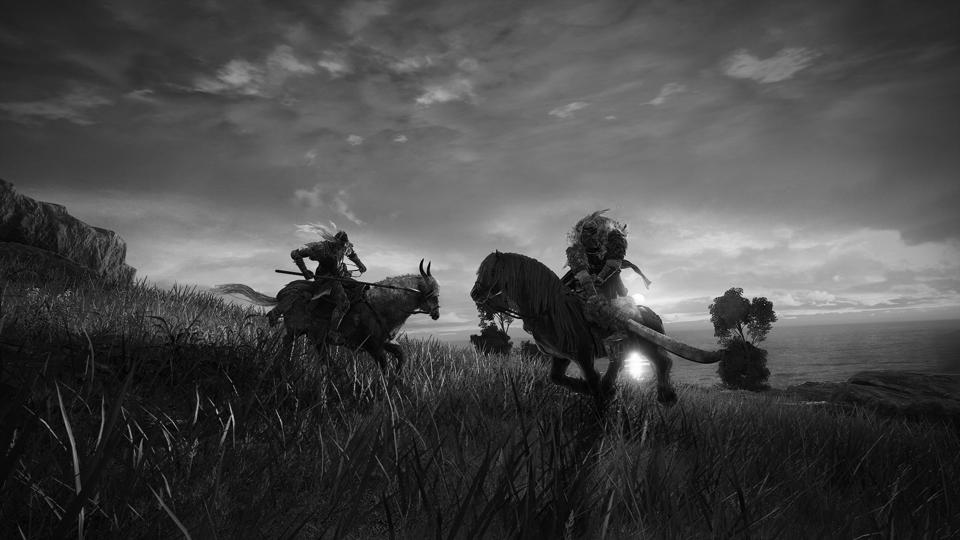
\includegraphics[width=8cm, height=4.5cm]{images/eldenring_grayscale.jpg}
    \caption{Original Gray scale Image}
\end{figure}

\subsection{Log Transformation}

Figure 2 contains the gray scale image after its been log transformed.

r is the input pixel, s is the output pixel, and c is a constant.

\begin{equation}
s=c\log{(1+r)}
\end{equation}

\begin{figure}[htbp]
    \centering
    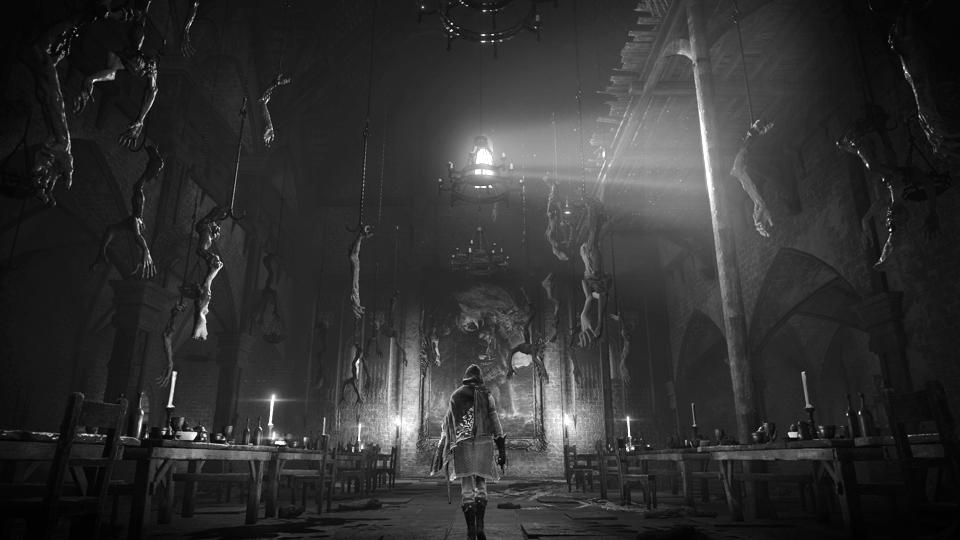
\includegraphics[width=8cm, height=4.5cm]{images/eldenring_log_transform.jpg}
    \caption{Log Transformation Image}
\end{figure}

The log transformation brightens the dark areas of the image. It stretch's the low intensity areas and compresses the high intensity areas. Here we can see the dark areas under the tables are more visible.

\subsection{Inverse Log Transformation}

Figure 3 contains the gray scale image after its been inverse log transformed.

r is the input pixel, s is the output pixel, and c is a constant.

\begin{equation}
s=c\log^{-1} (r)
\end{equation}

\begin{figure}[htbp]
    \centering
    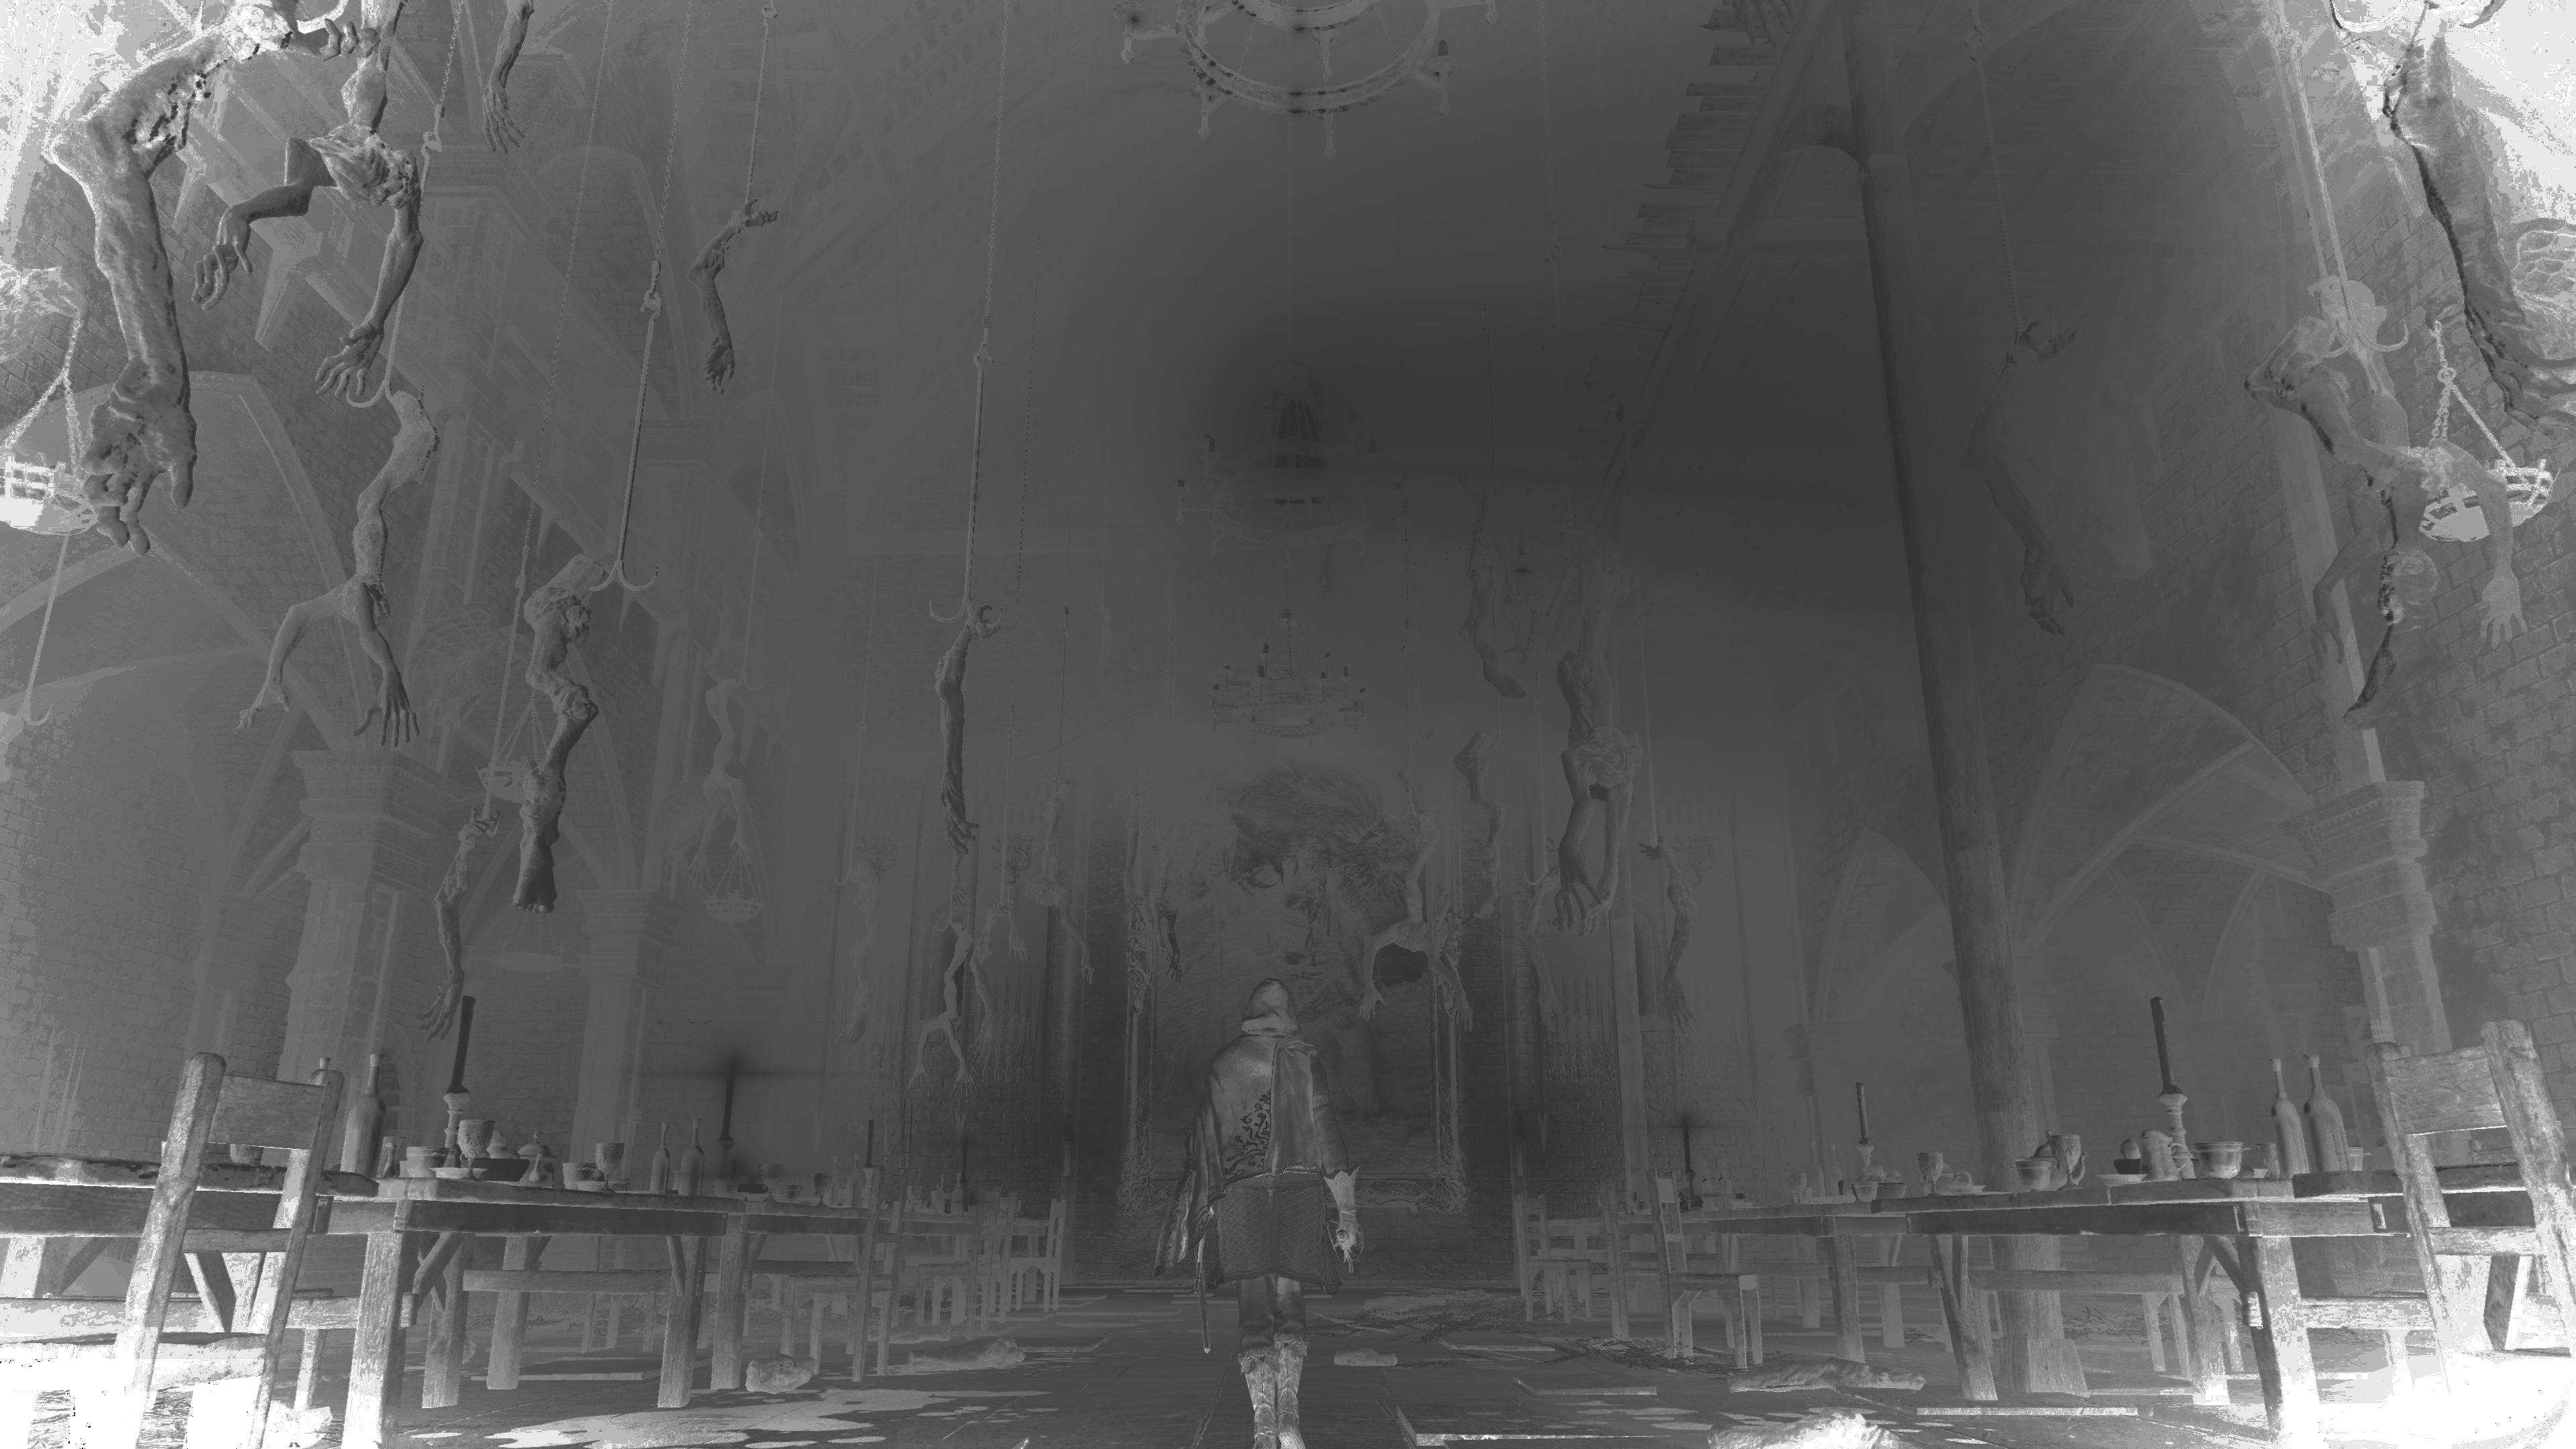
\includegraphics[width=8cm, height=4.5cm]{images/eldenring_inverse_log_transform.jpg}
    \caption{Inverse Log Transformation Image}
\end{figure}

The inverse log transformation darkens the dark areas of the image. It stretch's the high intensity areas and compresses the low intensity areas. Here we can see the dark areas under the tables are even less visible.

\subsection{Power Law Transformation}

Figure 4 contains the gray scale image after its been power law transformed with gamma as 3.

Figure 5 contains the gray scale image after its been power law transformed with gamma as 0.3.

\hfill

r is the input pixel, s is the output pixel, c and gamma is a constant.

\begin{equation}
s=cr^\gamma
\end{equation}

\begin{figure}[htbp]
    \centering
    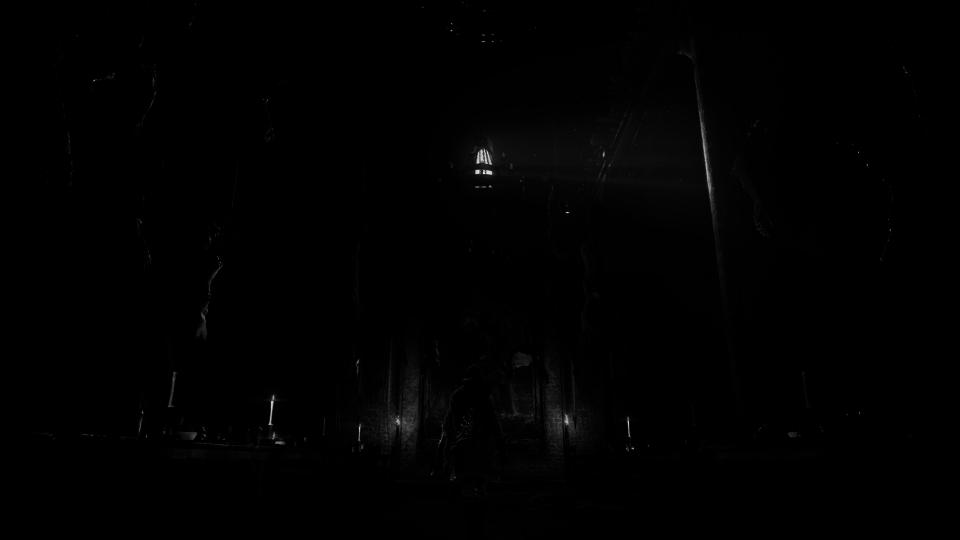
\includegraphics[width=8cm, height=4.5cm]{images/eldenring_power_law_blacken.jpg}
    \caption{Power law Transformation Image (gamma is 3)}
    \centering
    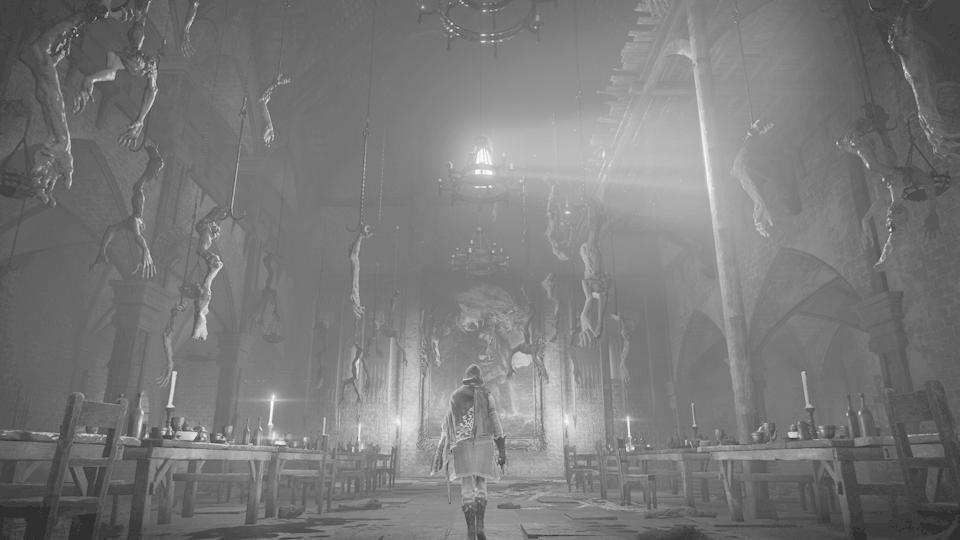
\includegraphics[width=8cm, height=4.5cm]{images/eldenring_power_law_whiten.jpg}
    \caption{Power law Transformation Image (gamma is 0.3)}
\end{figure}

With gamma as 3 we see the transformation work similar to inverse log transformation. With gamma as 0.3 we see the transformation work similar to the log transformation.

\section*{Part 1 - Problem 2}

In figure 6, the 8-bit place slicing is shown for the image.

The highest 4-bit and 2-bit planes reconstruction images are show in figure 7 and 8 respectively.

The 4-bit reconstruction shows more detail than the 2-bit reconstruction. Also, the 4-bit reconstruction is more discernible than the 2-bit reconstruction image.

\begin{figure}
    \begin{tabular}{cc}
        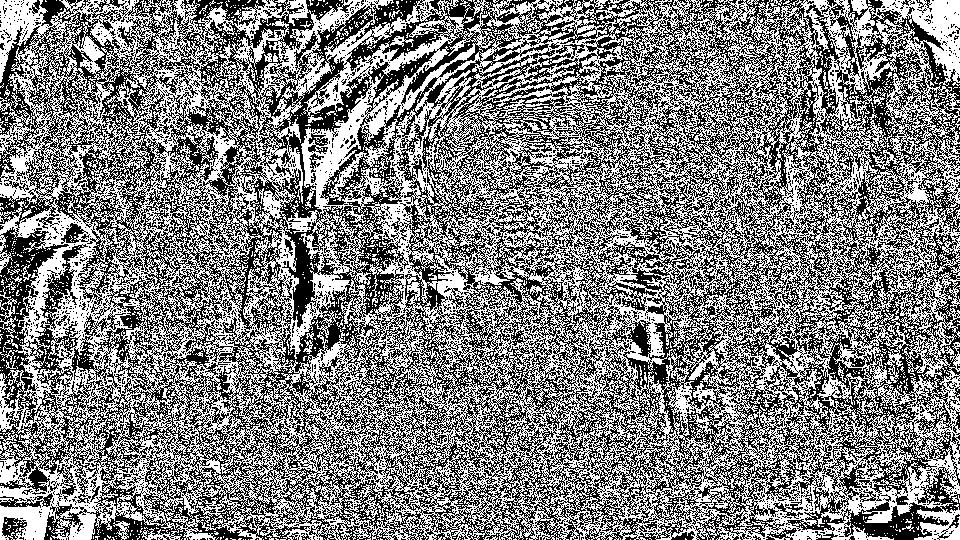
\includegraphics[width=4cm]{images/eldenring_1.jpg} & 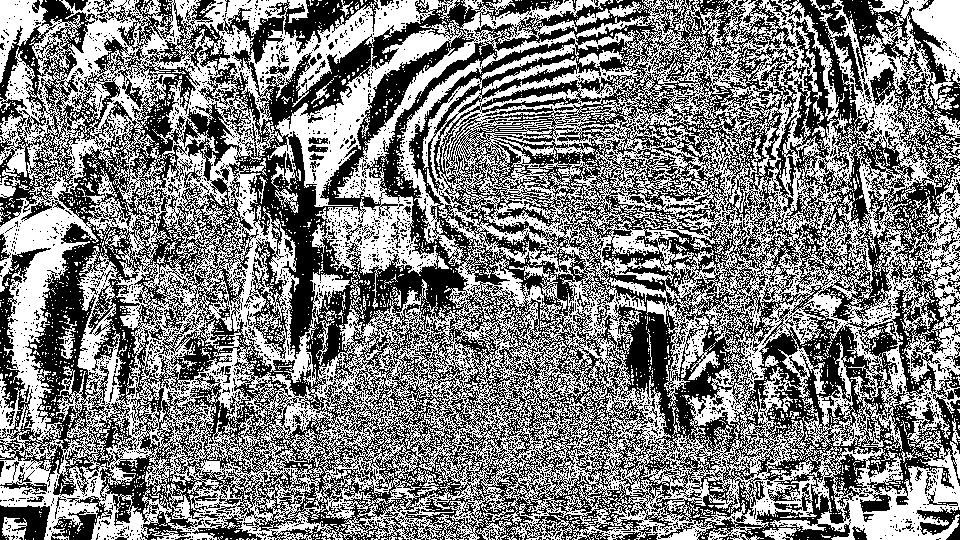
\includegraphics[width=4cm]{images/eldenring_2.jpg} \\  
        (a) Bit 1 & (b) Bit 2 \\[6pt]
        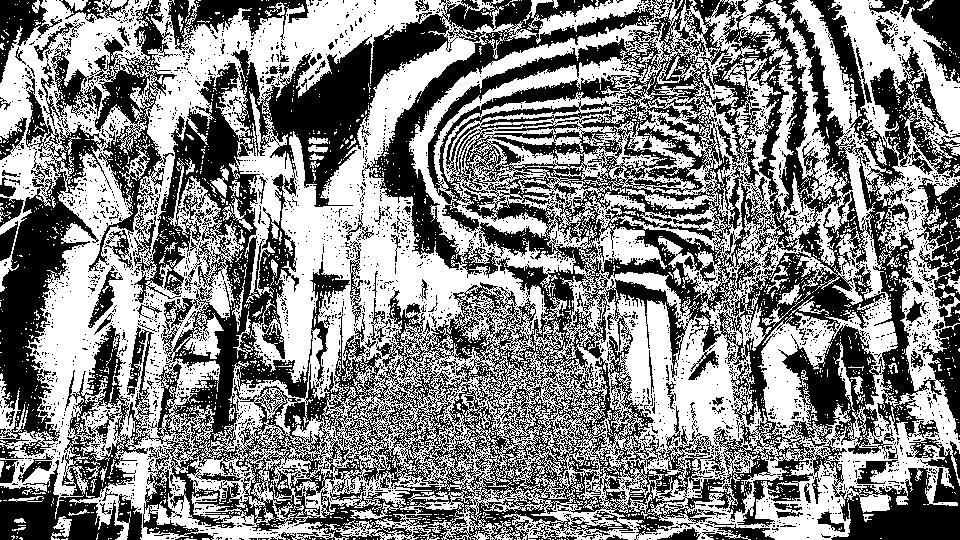
\includegraphics[width=4cm]{images/eldenring_3.jpg} & 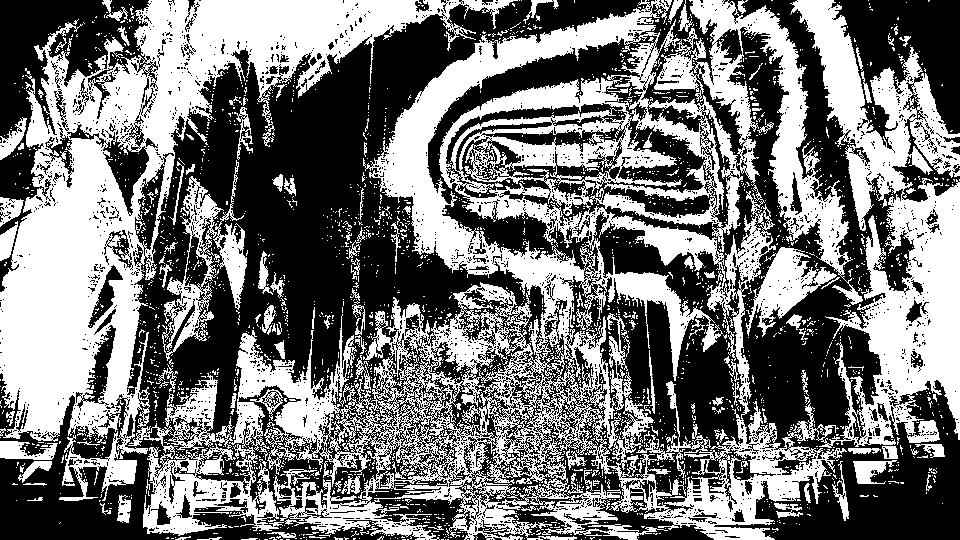
\includegraphics[width=4cm]{images/eldenring_4.jpg} \\
        (c) Bit 3 & (d) Bit 4 \\[6pt]
        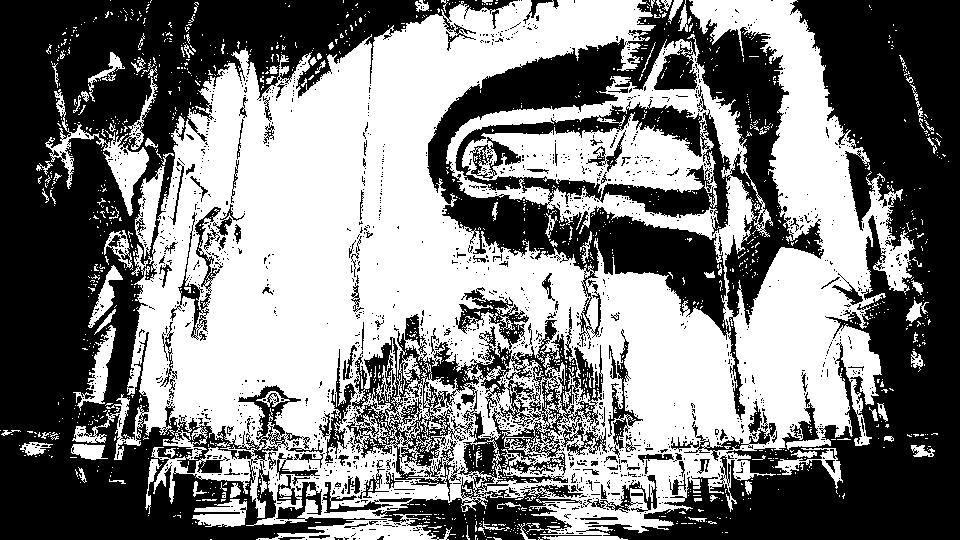
\includegraphics[width=4cm]{images/eldenring_5.jpg} & 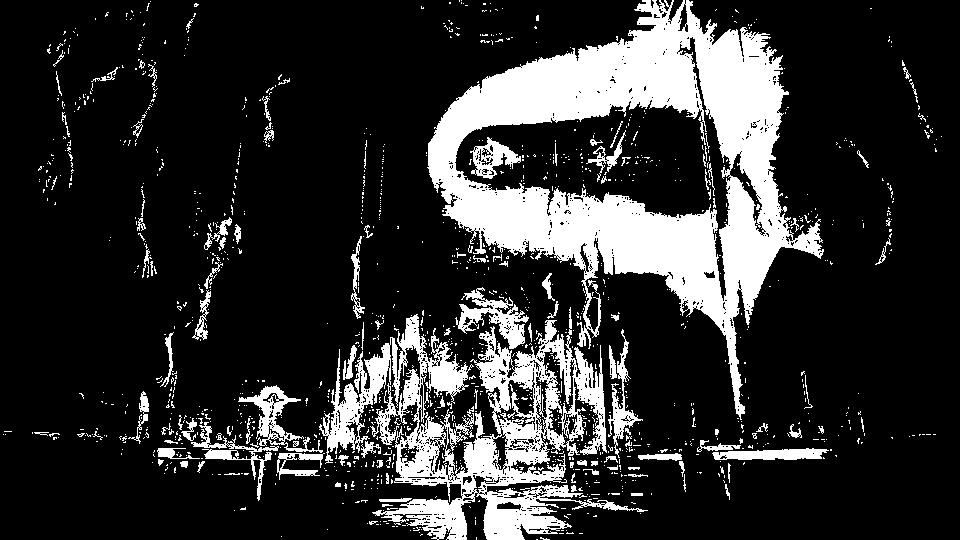
\includegraphics[width=4cm]{images/eldenring_6.jpg} \\  
        (a) Bit 5 & (b) Bit 6 \\[6pt]
        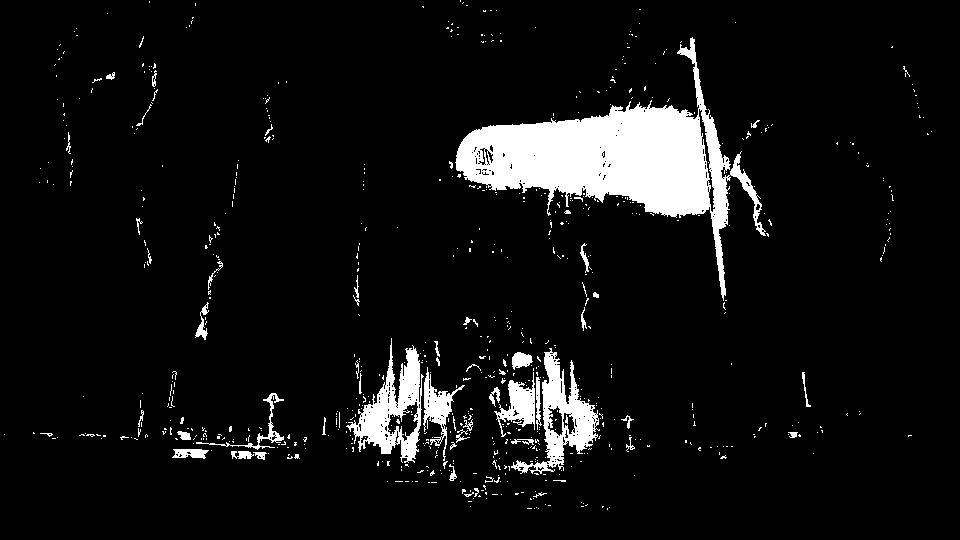
\includegraphics[width=4cm]{images/eldenring_7.jpg} & 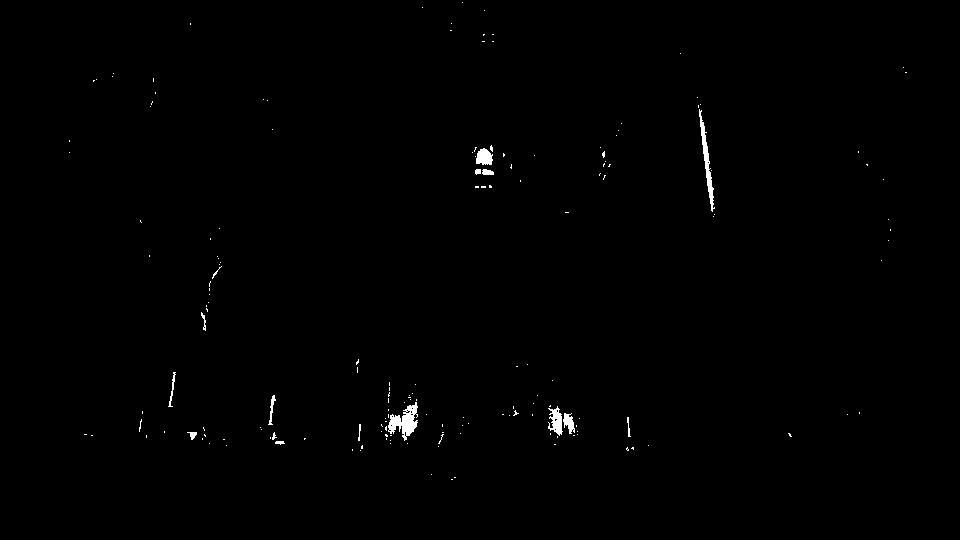
\includegraphics[width=4cm]{images/eldenring_8.jpg} \\  
        (a) Bit 7 & (b) Bit 8 \\[6pt]
        %\multicolumn{2}{c}{\includegraphics[width=65mm]{it} }\\
        %\multicolumn{2}{c}{(e) Bit 5}
    \end{tabular}
    \caption{8-Bit Place Slicing}
\end{figure}

\begin{figure}[htbp]
    \centering
    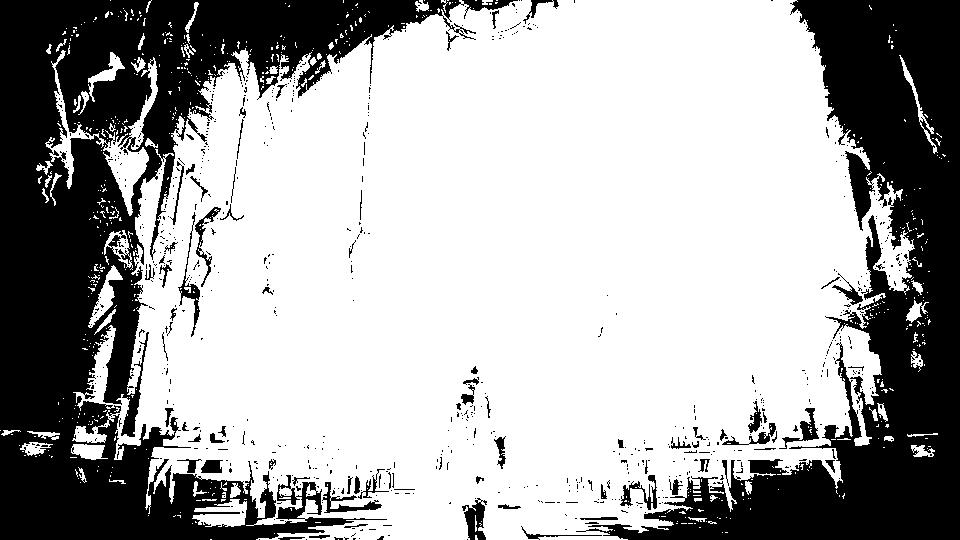
\includegraphics[width=8cm, height=4.5cm]{images/eldenring_5678.jpg}
    \caption{Highest 4-bit Reconstruction Image}
    \centering
    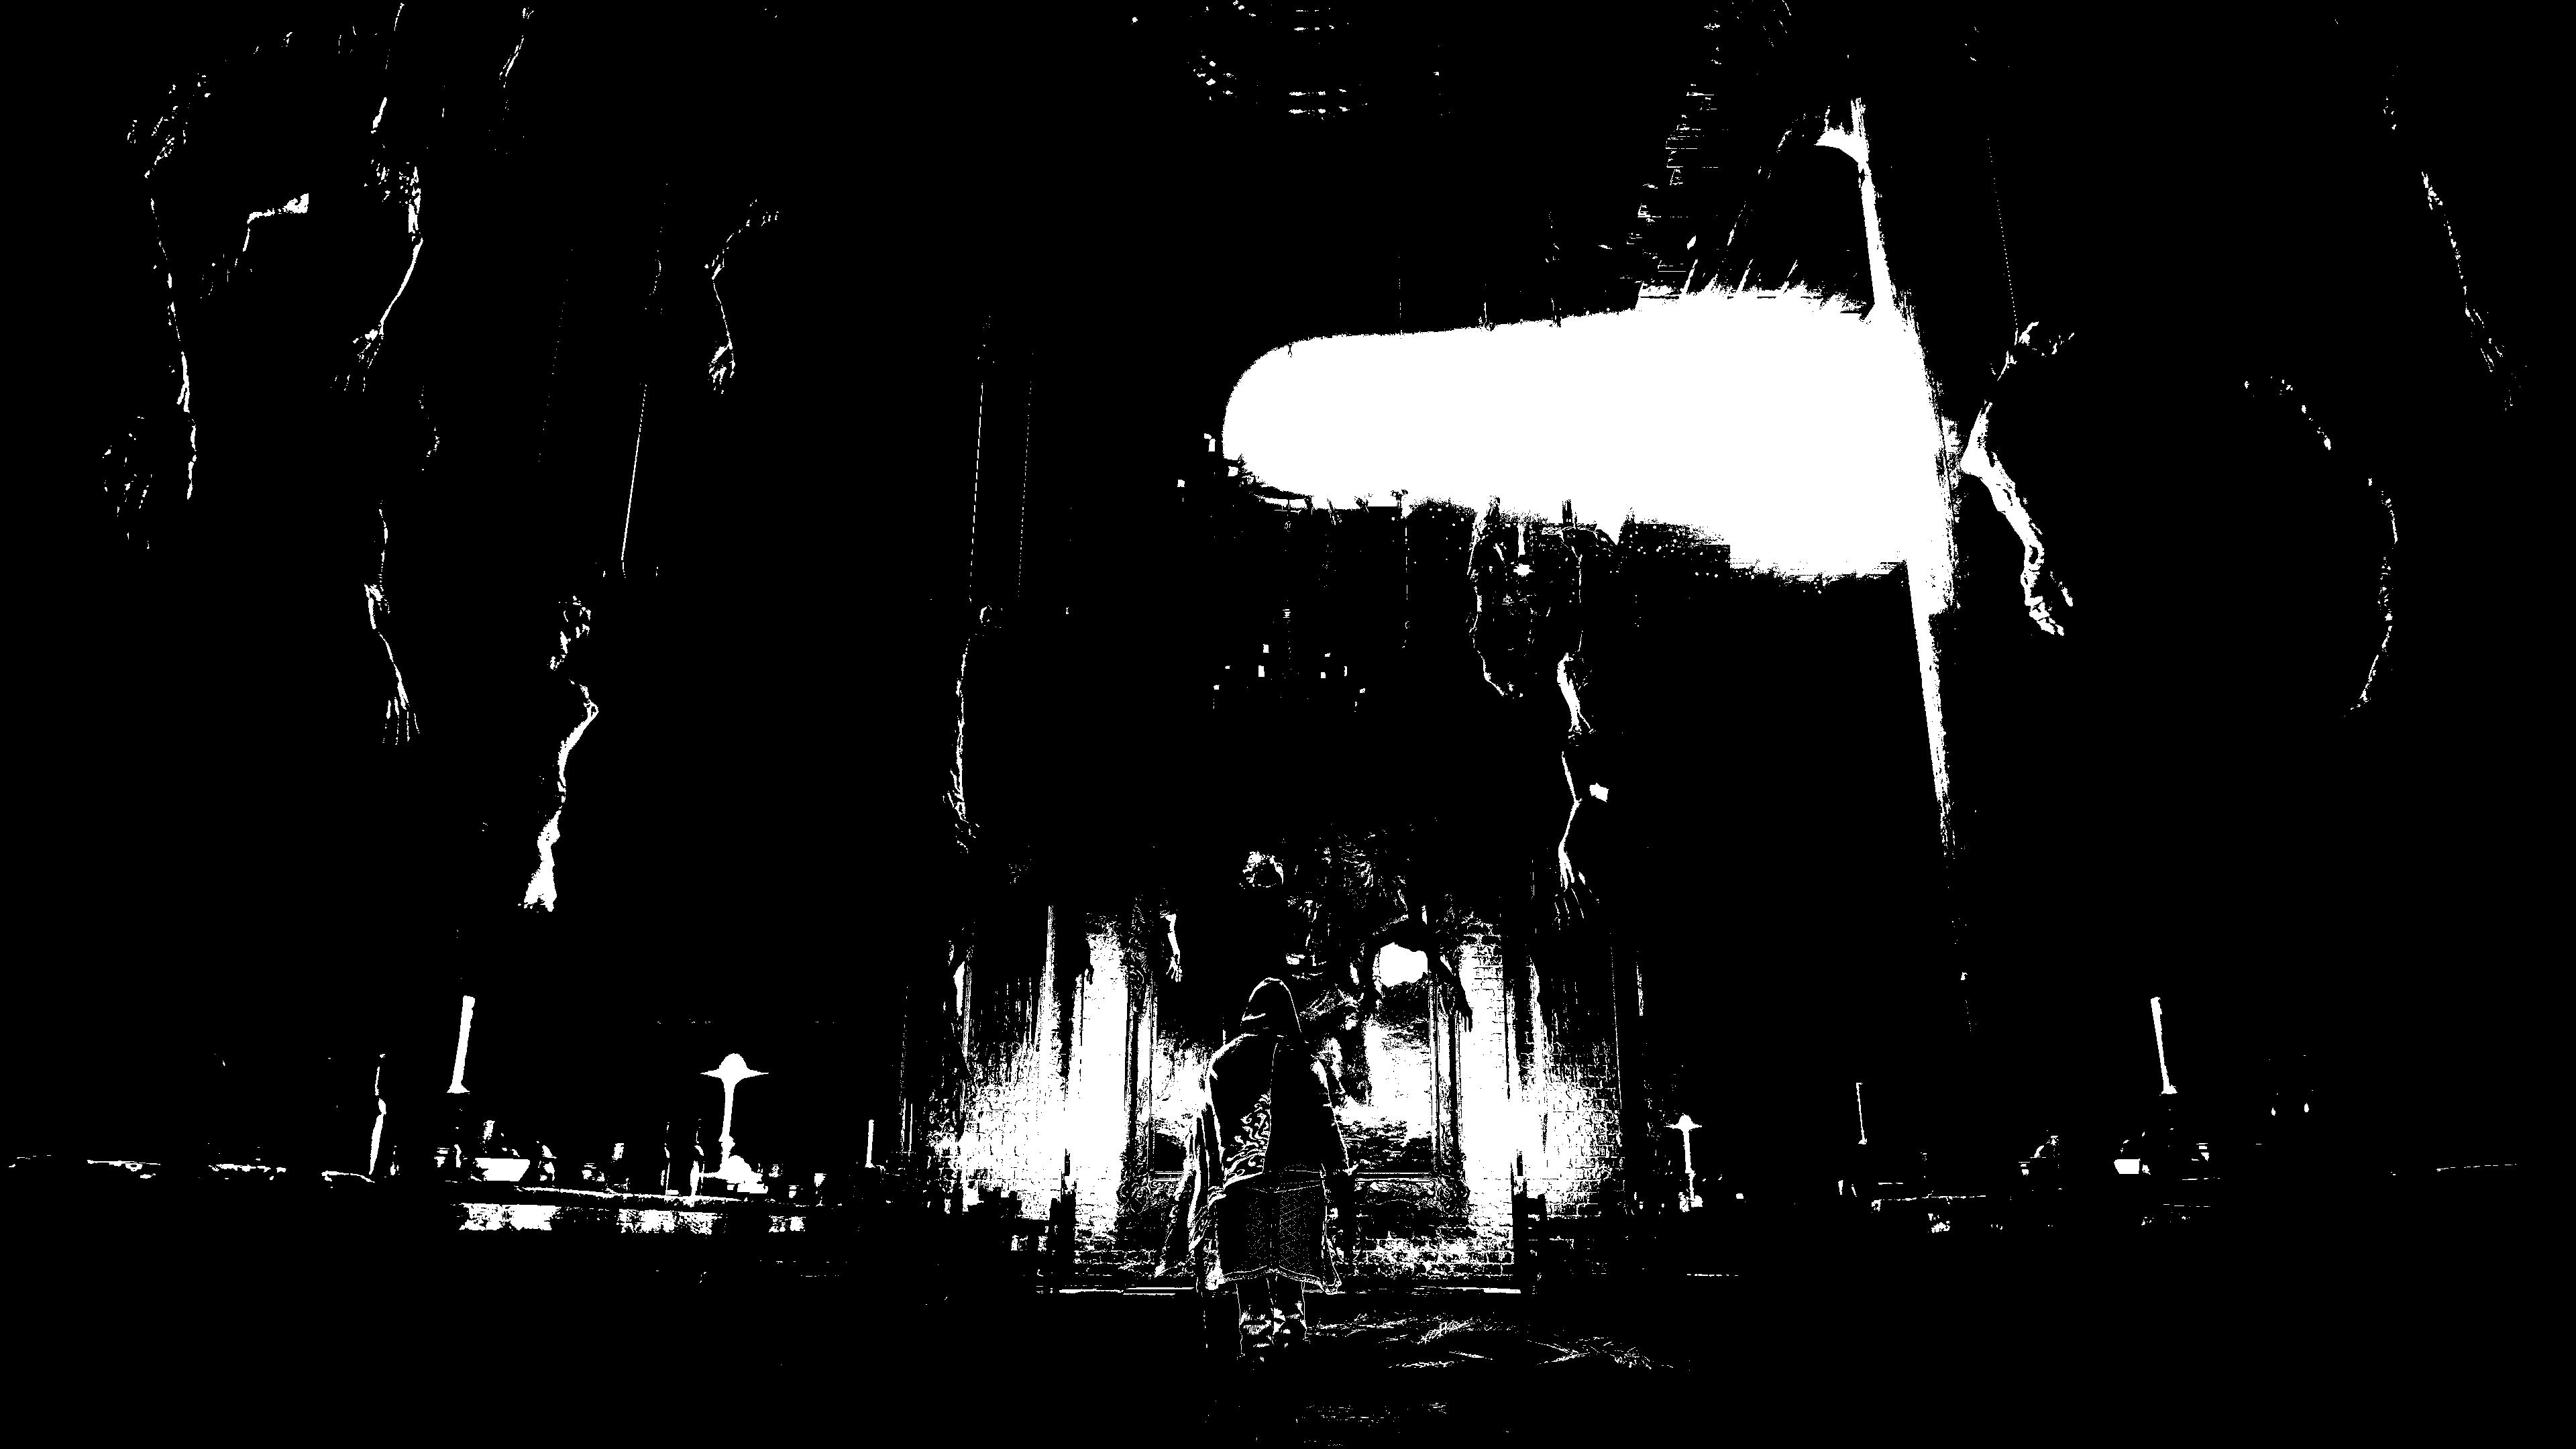
\includegraphics[width=8cm, height=4.5cm]{images/eldenring_78.jpg}
    \caption{Highest 2-bit Reconstruction Image}
\end{figure}

\section*{Part 1 - Problem 3}

Figure 9 shows the histograms of the original image and the power-law images, before and after they are histogram equalized.
\bigbreak
Figure 9a is the image histogram before equalization and Figure 9b is the image histogram after equalization. Before the image is clustered to lower intensities and after equalization it is more spread out.
\bigbreak
Figure 9c is the power law transformed(gamma=0.3) image histogram before equalization and Figure 9d is the power law transformed(gamma=0.3) image histogram after equalization. Before equalization the image has the intensities clustered in the middle and after it is is spread out just like 9b.
\bigbreak
Figure 9e is the power law transformed(gamma=3) image histogram before equalization and Figure 9f is the power law transformed(gamma=3) image histogram after equalization. Before equalization the image is very dark hence the it has very low intensity. After equalization, the image has higher intensity and is more spread out.
\bigbreak

\begin{figure}
    \begin{tabular}{cc}
        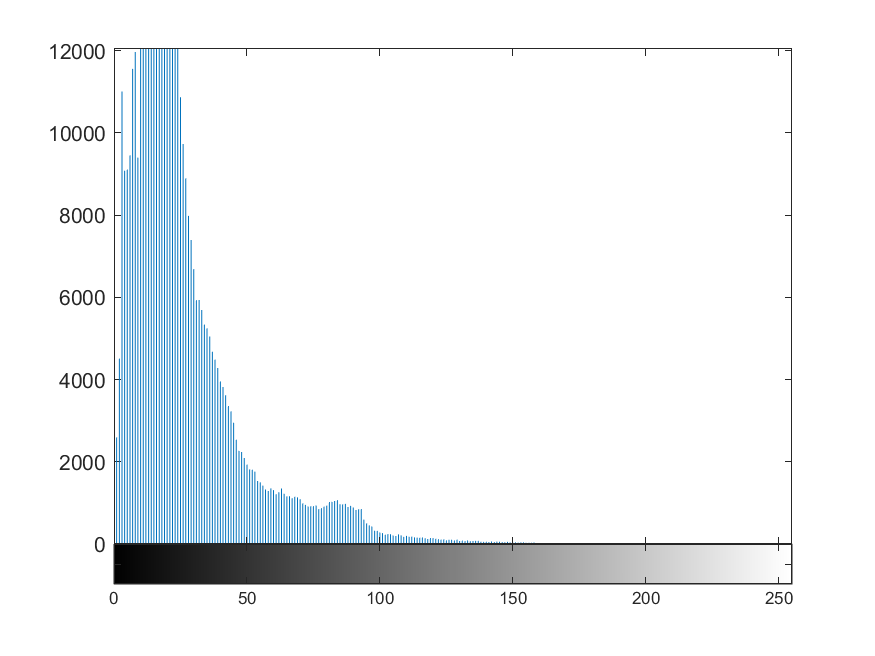
\includegraphics[width=3cm]{images/original_pre_hist.png} \\
        (a) Before-Original Image \\ [2pt]
        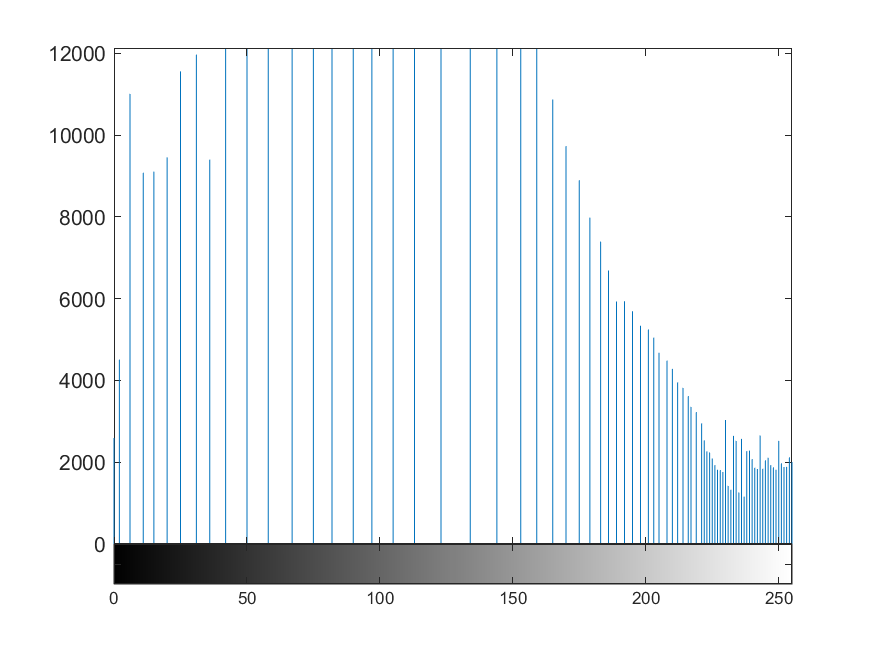
\includegraphics[width=3cm]{images/original_post_hist.png} \\
        (b) After-Original Image \\[2pt]
        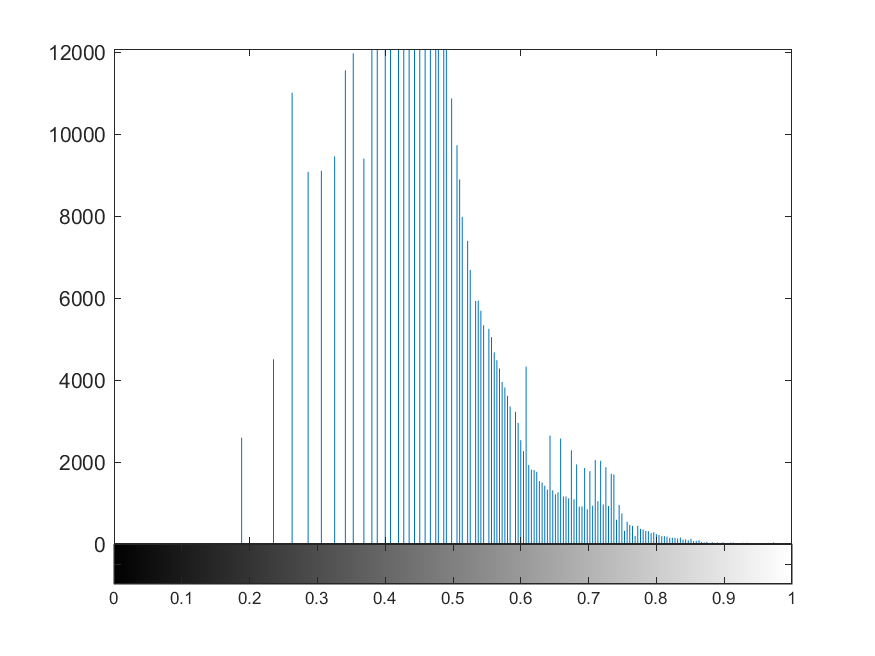
\includegraphics[width=3cm]{images/power_1_pre_hist.png} \\
        (c) Before-Power Law (gamma=0.3) \\[2pt]
        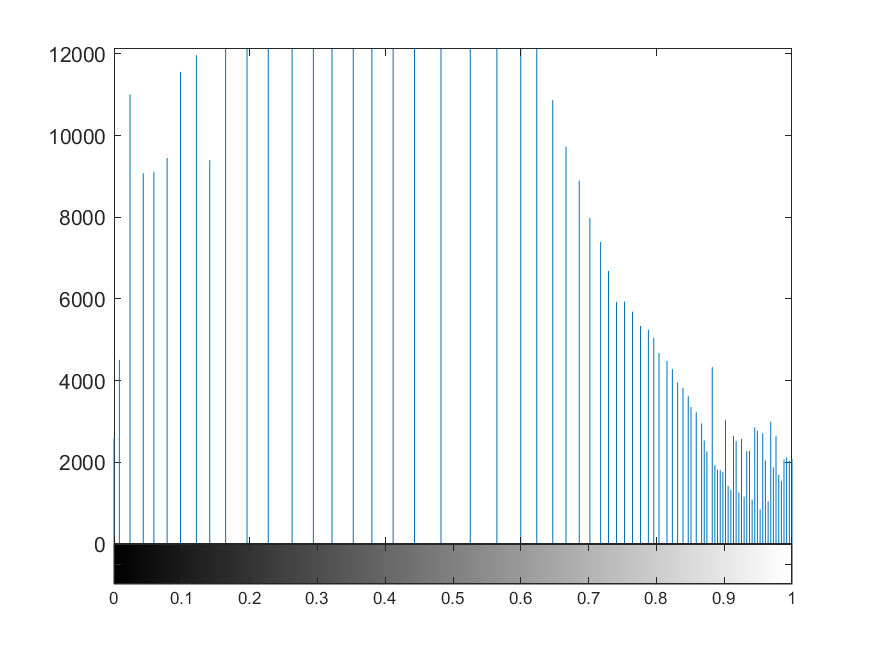
\includegraphics[width=3cm]{images/power_1_post_hist.png} \\
        (d) After-Power Law (gamma=0.3) \\[2pt]
        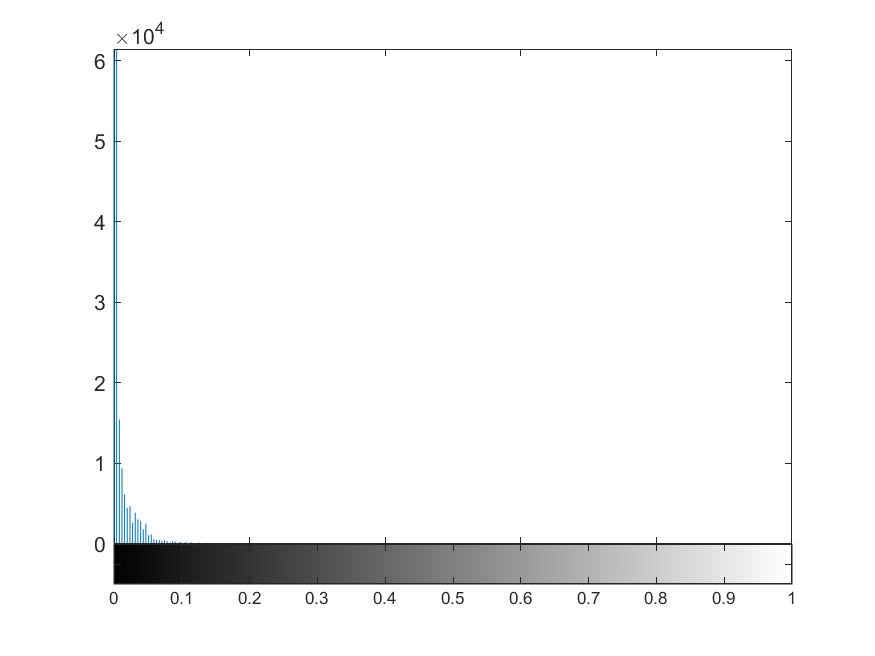
\includegraphics[width=3cm]{images/power_2_pre_hist.png} \\
        (e) Before-Power Law (gamma=3) \\[2pt]
        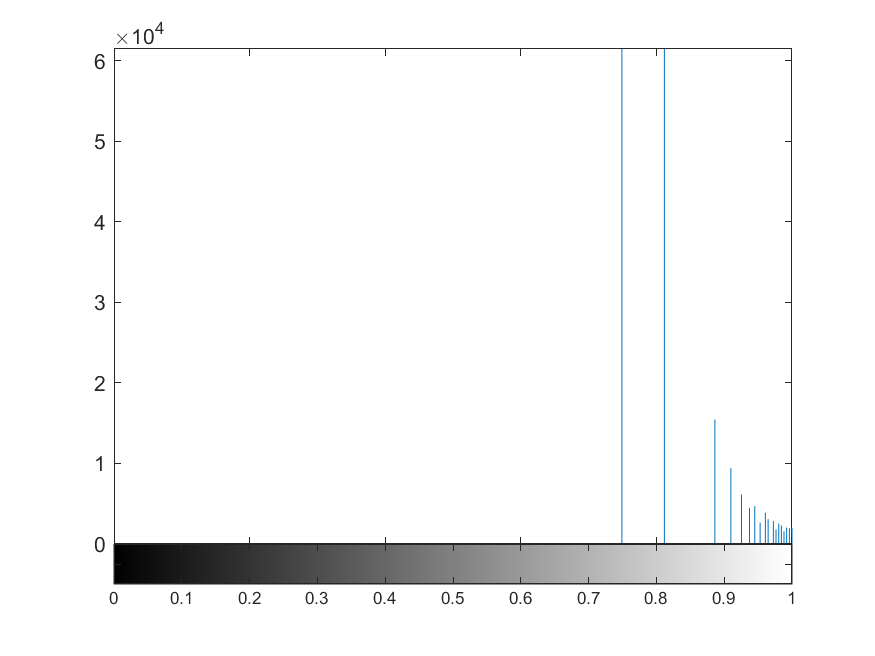
\includegraphics[width=3cm]{images/power_2_post_hist.png} \\
        (f) After-Power Law (gamma=3) \\[2pt]
    \end{tabular}
    \caption{Before and After Histogram Equalization}
\end{figure}

\section*{Part 1 - Problem 4}

Histogram matching is a transformation of an image to make its histogram match another histogram.

The procedure for histogram matching is as follows:
\begin{itemize}
  \item First we get the probability distribution of the input data p\textsubscript{r}(r\textsubscript{k})
  \item Second, do Histogram Equalization on input $s=T(r)$, where T is the histogram equalization.
  \item Thirdly, we compute $s=G(z)$.
  \item After, we get the inverse mapping $z=G^{-1}(s)$.
  \item The output image with values z is the histogram matched image.
\end{itemize}

You will not obtain the same histogram as the desired one after histogram matching because of rounding to discrete values that happens during histogram equalization.

\section*{Part 1 - Problem 5}

The histogram before equalization is shown in Figure 10, while the histogram after equalization is shown in Figure 11.

The calculation of histogram equalization is as follows: 
\hfill

\begin{center}
\begin{tabular}{ |c|c|c|c|c| } 
\hline
r\textsubscript{k} & n\textsubscript{k} & p\textsubscript{r}(r\textsubscript{k}) = n\textsubscript{k}/MN & s\textsubscript{k} & Rounded s\textsubscript{k}\\
\hline
r\textsubscript{0} = 0 & 0 & 0 & s\textsubscript{0} = 0 & s\textsubscript{0} = 0\\ 
r\textsubscript{1} = 1 & 7 & 0.35 & s\textsubscript{1} = 2.45 & s\textsubscript{1} = 2\\
r\textsubscript{2} = 2 & 3 & 0.15 & s\textsubscript{2} = 3.50 & s\textsubscript{2} = 4\\
r\textsubscript{3} = 3 & 2 & 0.10 & s\textsubscript{3} = 4.20 & s\textsubscript{3} = 4\\
r\textsubscript{4} = 4 & 3 & 0.15 & s\textsubscript{4} = 5.25 & s\textsubscript{4} = 5\\
r\textsubscript{5} = 5 & 1 & 0.05 & s\textsubscript{5} = 5.60 & s\textsubscript{5} = 6\\
r\textsubscript{6} = 6 & 1 & 0.05 & s\textsubscript{6} = 5.95 & s\textsubscript{6} = 6\\
r\textsubscript{7} = 7 & 3 & 0.15 & s\textsubscript{7} = 7.00 & s\textsubscript{7} = 7\\
\hline
\end{tabular}
\end{center}

\begin{figure}[htbp]
    \centering
    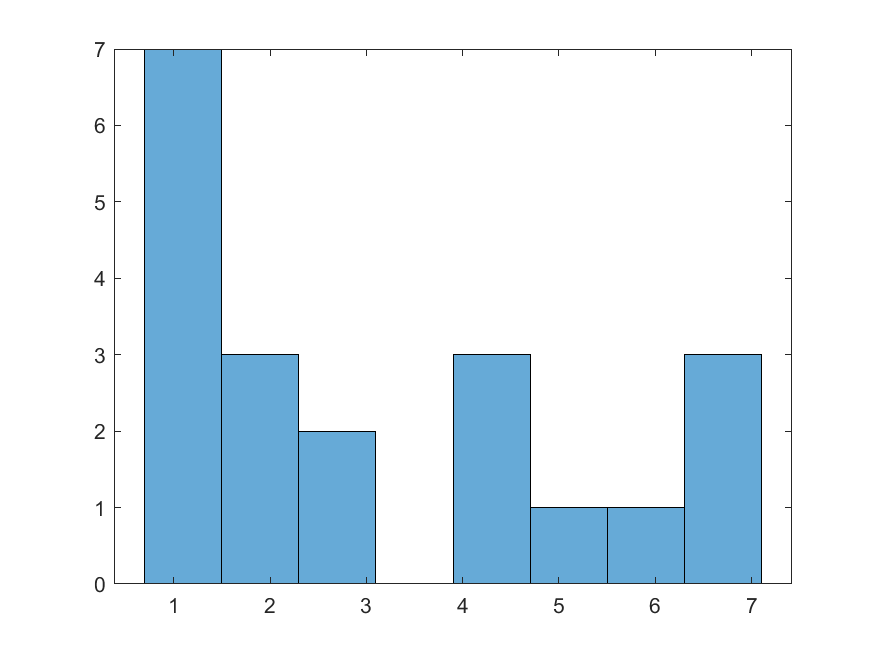
\includegraphics[width=8cm, height=4.5cm]{images/manual_pre_hist.png}
    \caption{Before Histogram Equalization}
    \centering
    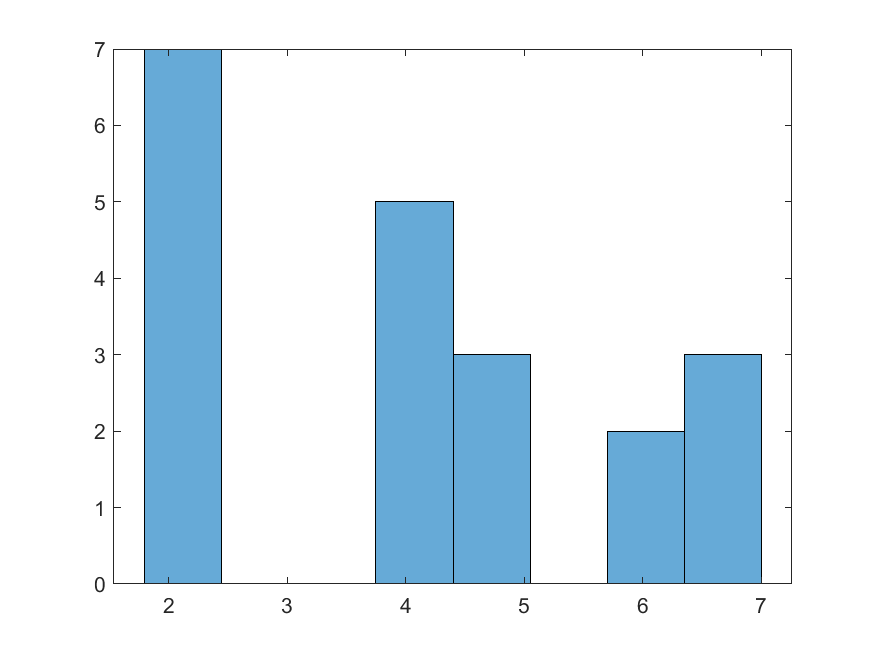
\includegraphics[width=8cm, height=4.5cm]{images/manual_post_hist.png}
    \caption{After Histogram Equalization}
\end{figure}

Before Histogram Equalization:

\begin{center}
\begin{tabular}{ |l|l|l|l|l| } 
\hline
1 & 2 & 4 & 7 & 3\\ \hline
2 & 4 & 7 & 3 & 1\\ \hline
5 & 6 & 2 & 1 & 1\\ \hline
4 & 7 & 1 & 1 & 1\\ \hline
\end{tabular}
\end{center}

After Histogram Equalization:

\begin{center}
\begin{tabular}{ |l|l|l|l|l| } 
\hline
2 & 4 & 5 & 7 & 4\\ \hline
4 & 5 & 7 & 4 & 2\\ \hline
6 & 6 & 4 & 2 & 2 \\ \hline
5 & 7 & 2 & 2 & 2\\ \hline
\end{tabular}
\end{center}

\section*{Part 2}

Explanation of each step for padding and shearing an image:
\begin{itemize}
  \item \textbf{Step 1:} We use simple shear to transform the image. Simple shear is an affine transformation, we make an affine with maketform with the simple shear matrix values. What shear does is it moves a point further away from an axis, the more further away it is from another axis, which creates a bent rotated like shape.
  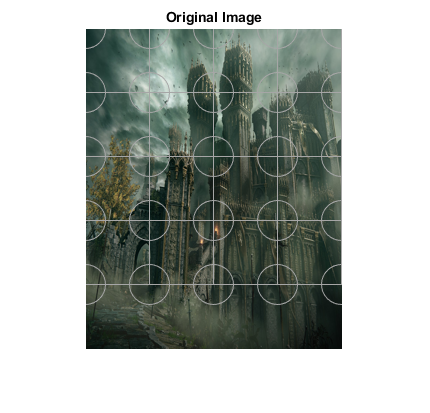
\includegraphics[width=8cm, height=4.5cm]{images/original.png}
  
  \item \textbf{Step 2:} Here we draw lines and circles to examine how the simple shear transformation affected these shapes. We can see the circles and lines have been bent according to the shear.
  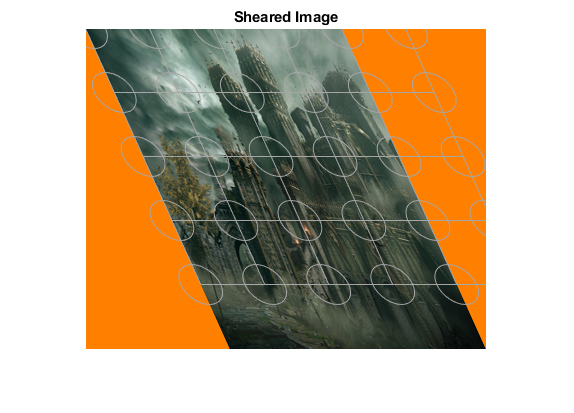
\includegraphics[width=8cm, height=4.5cm]{images/sheared.png}
  
  \item \textbf{Step 3:} We compare different padding options, for "fill" we simply feel with a orange static color. Replicate padding makes a copy of the input, reverses it and applies that as the padding. Bound padding applies a strict distinction between the padding and the input. Bound has clear boundaries compared to fill method.
  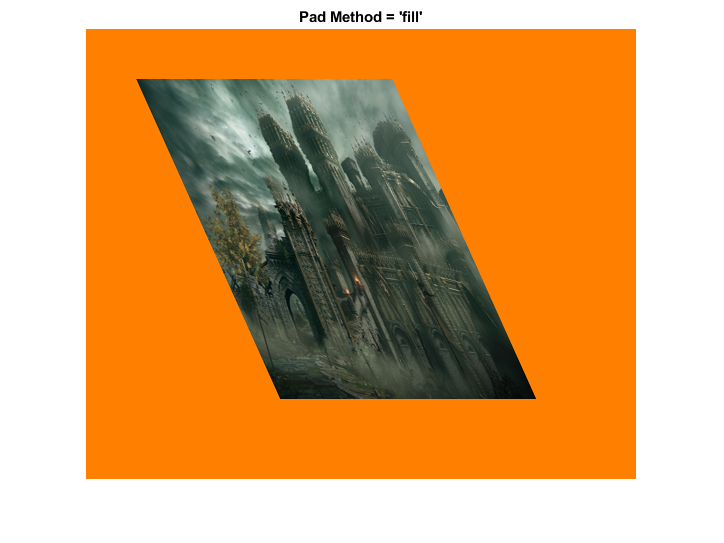
\includegraphics[width=8cm, height=4.5cm]{images/transformation_fill.png}
  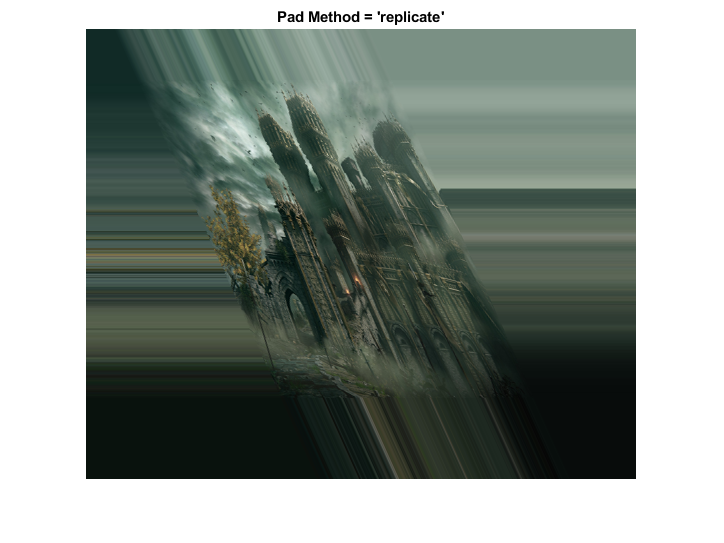
\includegraphics[width=8cm, height=4.5cm]{images/transformation_replicate.png}
  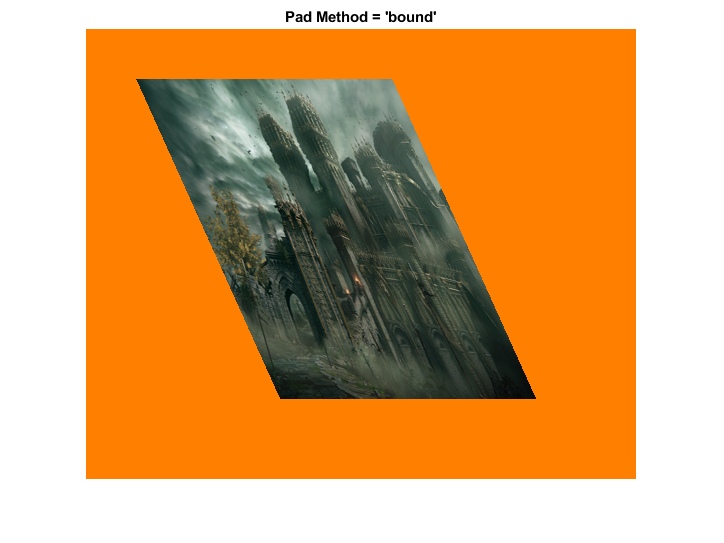
\includegraphics[width=8cm, height=4.5cm]{images/transformation_bound.png}
  
  \item \textbf{Step 4:} Here we try two padding methods, circular and symmetric. The circular method takes copies of the image and replicates it. The symmetric method takes the mirror of the image and fills padding with it.
  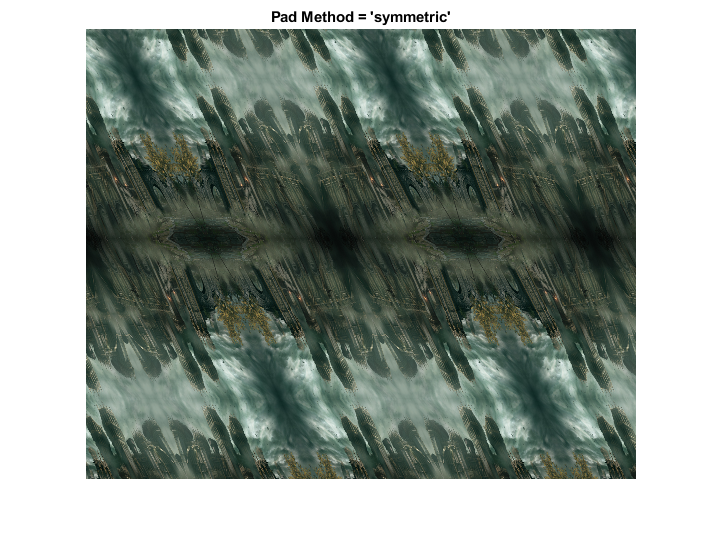
\includegraphics[width=8cm, height=4.5cm]{images/transform_symmetric.png}
  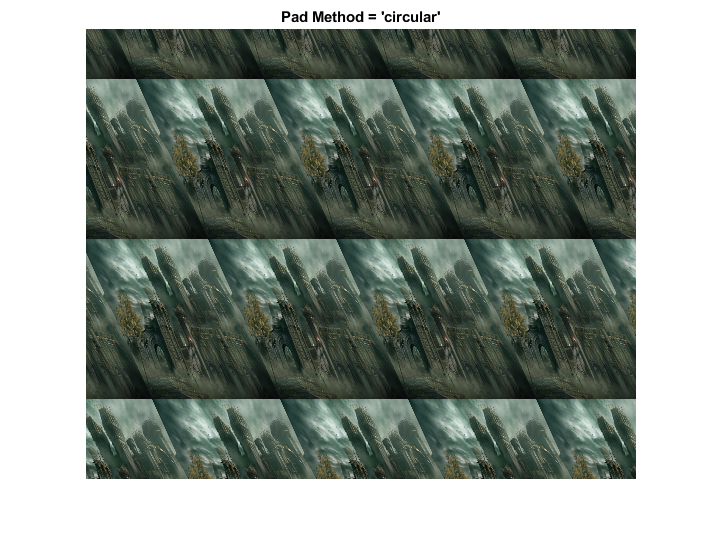
\includegraphics[width=8cm, height=4.5cm]{images/transformation_circular.png}
  
\end{itemize}

\begin{thebibliography}{00}
\bibitem{b1} Code for this assignment at ./a1.m
\bibitem{b2} Assignment source code: \url{https://github.com/UdbhavPrasad072300/CPS843-Assignments}
\end{thebibliography}

\end{document}
